
% ==================================================
% 1. CLASSE DEL DOCUMENT
% ==================================================
\documentclass[a4paper,11pt,oneside]{article}

% ==================================================
% 2. PAQUETS ESSENCIALS (IDIOMA I CODIFICACIÓ)
% ==================================================
\usepackage[utf8]{inputenc}
\usepackage[T1]{fontenc}
\usepackage[catalan]{babel}
\usepackage{lmodern}

% ==================================================
% 3. FORMAT DEL TEXT I DELS PARÀGRAFS
% ==================================================
\setlength{\parindent}{0.5cm}
\usepackage{indentfirst}

\usepackage{setspace}
\singlespacing

% ==================================================
% 4. MATEMÀTIQUES
% ==================================================
\usepackage{amsmath,amssymb,amsthm}
\usepackage{mathtools}
\usepackage{bm}
\usepackage{siunitx}

% ==================================================
% 5. DISSENY I FORMAT DE LA PÀGINA
% ==================================================
\usepackage{geometry}
\geometry{
    a4paper,
    margin=2.5cm,
    top=2.5cm,
    bottom=2.5cm
}

\raggedbottom

% ==================================================
% 6. TÍTOLS I SECCIONS
% ==================================================
\usepackage{titlesec}

% Format de les seccions principals
\titleformat{\section}
  {\normalfont\Large\bfseries}
  {\thesection.}
  {0.5em}
  {}

% Format de les subseccions
\titleformat{\subsection}
  {\normalfont\large\bfseries}
  {\thesubsection.}
  {0.5em}
  {}

% Format de les subsubseccions
\titleformat{\subsubsection}
  {\normalfont\normalsize\bfseries}
  {\thesubsubsection.}
  {0.5em}
  {}

% Espaiats dels títols
\titlespacing*{\section}{0pt}{18pt}{10pt}
\titlespacing*{\subsection}{0pt}{12pt}{6pt}
\titlespacing*{\subsubsection}{0pt}{8pt}{4pt}

% ==================================================
% 7. CAPÇALERES I PEUS DE PÀGINA
% ==================================================

% ==================================================
% CAPÇALERES I PEUS DE PÀGINA
% ==================================================

\usepackage{fancyhdr}

\pagestyle{fancy}
\fancyhf{}

% Mostrar el número i el nom de la secció
\renewcommand{\sectionmark}[1]{%
    \markboth{\thesection.\ #1}{}
}

% Capçalera: nom de la secció a l'esquerra
\fancyhead[L]{\nouppercase{\leftmark}}

% Número de pàgina centrat al peu
\fancyfoot[C]{\thepage}

% Línies de capçalera i peu
\renewcommand{\headrulewidth}{0.4pt}
\renewcommand{\footrulewidth}{0pt}

% Configuració de les pàgines plain
\fancypagestyle{plain}{
    \fancyhf{}
    \fancyhead[L]{\nouppercase{\leftmark}}
    \fancyfoot[C]{\thepage}
    \renewcommand{\headrulewidth}{0.4pt}
    \renewcommand{\footrulewidth}{0pt}
}

% ==================================================
% 8. GRÀFICS, TAULES I COLORS
% ==================================================
\usepackage{graphicx}
\usepackage[table]{xcolor}
\usepackage{array}
\usepackage{tabularx}
\usepackage{multirow}
\usepackage{booktabs}
\usepackage{makecell}
\usepackage{float}
\usepackage[font=small]{caption}
\usepackage{subcaption}

% Caixes de text
\usepackage{tcolorbox}
\tcbuselibrary{most}

% Colors
\definecolor{grisC}{RGB}{211,211,211}
\definecolor{grisF}{gray}{0.3}

% ==================================================
% 9. ENLLAÇOS I REFERÈNCIES
% ==================================================
\usepackage[hidelinks]{hyperref}
\usepackage{bookmark}

\usepackage[autostyle]{csquotes}
\DeclareQuoteStyle{catalan}
  {\guillemotleft}{\guillemotright}
  {\quotesinglbase}{\guillemotright}

\usepackage[
    backend=biber,
    style=numeric,
    sorting=none
]{biblatex}

% ==================================================
% 10. ALTRES PAQUETS ÚTILS
% ==================================================
\usepackage{varwidth}
\usepackage{enumitem}
\usepackage[title,titletoc]{appendix}

% ==================================================
% 11. CONFIGURACIÓ D'ENTORNS DE TEOREMES
% ==================================================
% \theoremstyle{definition}
% \newtheorem{definicio}{Definició}[section]
%
% \theoremstyle{plain}
% \newtheorem{teorema}{Teorema}[section]
% \newtheorem{propietat}{Propietat}[section]
%
% \theoremstyle{remark}
% \newtheorem{exemple}{Exemple}[section]
% \newtheorem{nota}{Nota}[section]

% ==================================================
% 12. INICI DEL DOCUMENT
% ==================================================
\begin{document}

\begin{titlepage}
    \thispagestyle{empty}
    \centering

    % Universitat
    \vspace*{1.5cm}

    {\Large\scshape Universitat Autònoma de Barcelona\par}
    \vspace{0.3cm}
    {\large Grau en Física\par}

    % Títol principal
    \vspace{2.5cm}

    {\color{gray}\rule{1\textwidth}{1.2pt}\par}

    \vspace{0.8cm}

    {\large\bfseries PRÀCTICA 1\par}

    \vspace{0.5cm}

    {\Huge\bfseries Modelització d'una ablació cardíaca IVS\par}

    \vspace{0.6cm}

    {\large INFORME DE PRÀCTIQUES\par}

    \vspace{0.8cm}

    {\color{gray}\rule{1\textwidth}{1.2pt}\par}

    % Dades dels grups
    \vspace{2cm}

    {\large\bfseries Grup 111\par}

    \vspace{0.8cm}

    {\large Gabriel Vicente Vitagliano Castan 1639230\par}
    \vspace{0.2cm}
    {\large Aleix Fosalba Pujols 1709441\par}
    \vspace{0.2cm}
    {\large Víctor Shenyu Lechuga Izquierdo 1753089\par}
    \vspace{0.2cm}
    

    % Informació inferior
    \vfill

    {\large\bfseries Mètodes Numèrics II\par}

    \vspace{0.3cm}

    {\large Curs acadèmic 2026--2027\par}

    \vspace{1cm}

\end{titlepage}

\newpage

\tableofcontents

\newpage

\section{Introducció}

L'ablació cardíaca és un procediment mèdic utilitzat per tractar arrítmies cardíaques mitjançant l'aplicació de calor. En 
aquesta pràctica s'estudia l'ablació cardíaca interventricular (IVS), basada en l'aplicació d'una diferència de potencial entre 
dos elèctrodes de polaritat oposada. Aquest procés genera calor per efecte Joule, augmentant la temperatura i destruint el 
teixit malalt.

L'objectiu principal és determinar el temps òptim d'aplicació d'una tensió alterna de 40 V $\text{(pi a pic)}$ sobre un teixit 
cardíac de 2 cm de gruix, amb una regió central de 0.5 cm corresponent al teixit malalt. El tractament ha de garantir que aquesta 
regió assoleixi temperatures superiors als 50 $^\circ$C, evitant que el teixit sa superi aquest llindar i que cap zona arribi als 80 $^\circ$C, 
per evitar complicacions mèdiques.

Per estudiar l'evolució temporal i espacial de la temperatura, es modelitza la transferència de calor mitjançant l'equació de 
Fourier en una dimensió, incorporant la generació de calor per efecte Joule. Es resol el model mitjançant tres mètodes numèrics: 
Euler explícit, Euler implícit i Crank-Nicolson. Es comparen els resultats obtinguts per als diferents mallats, estudiant-ne 
l'error numèric, l'estabilitat i la precisió, amb la finalitat de determinar les condicions més adequades per dur a terme el 
tractament.

\section{Mètodes numèrics}

\subsection{Normalització}

La llei de Fourier per la temperatura és:

\begin{equation}
    c_v \rho \dfrac{\partial T}{\partial x} = \nabla (\kappa \nabla T) + P_{\text{ext}},
    \label{fourier}
\end{equation}

on $c_v$ és el calor específic, $\rho$ és la densitat, $\kappa$ és la conductivitat tèrmica i $P_{\text{ext}}$ representa totes 
les fonts de calor externes. Per aquest problema considerarem que l'única font de calor externa és la calor produïda pels 
elèctrodes que generen calor per efecte Joule.

A continuació definim les variables normalitzades:

\begin{equation}
    \widetilde{T}=\frac{T}{T_0};\quad \widetilde{x}=\frac{x}{x_0};\quad \widetilde{t}=t/t_0
    \label{norm}
\end{equation}
d'on trobem l'equació:
\begin{equation*}
    \frac{\partial \widetilde{T}}{\partial \widetilde{t}} = \frac{\partial^2 \widetilde{T}}{\partial \widetilde{x}^2}  
    \frac{t_0\kappa}{x_0^2c_v\rho}+\frac{\sigma (\Delta V)^2t_0}{T_0d^2c_v\rho}
\end{equation*}
I en particular:
 \begin{equation}
     x_0=d \quad t_0=\frac{d^2}{\alpha} \quad T_0=\frac{\sigma (\Delta V)^2}{\kappa}
\end{equation}

Ara ja podem renormalitzar l'equació (\ref{fourier}). La llei de Fourier normalitzada és:

\begin{equation}
    \frac{\partial \widetilde{T}}{\partial \widetilde{t}}=\frac{\partial^2 \widetilde{T}}{\partial \widetilde{x}^2} + 1
    \label{fouriernorm}
\end{equation}

La renormalització ens ha permès reduir el nombre de paràmetres del problema expressant les variables en forma adimensional. Això 
simplifica l'equació diferencial, facilita els càlculs numèrics i permet comparar diferents sistemes físics independentment de 
les seves unitats de mesura.

La difusivitat tèrmica, definida com $\alpha=\frac{\kappa}{c_v\rho}$, determina la rapidesa amb què la calor es propaga a través 
del teixit. Depèn de la conductivitat tèrmica, la calor específica i la densitat del material. Com més gran és la difusivitat, 
més ràpidament es transmeten les variacions de temperatura. En el nostre sistema, determina l'escala temporal característica del 
procés de difusió tèrmica i, per tant, influeix directament en la durada del tractament.

Els valors numèrics emprats en aquesta pràctica són els següents: 
\begin{equation*}
    c_v = 3698 \ \frac{\text{J}}{\text{kg \ K}}, \quad \rho = 1081 \ \frac{\text{kg}}{\text{m} ^3}, \quad \kappa = 0.56 \ \frac{\text{W}}{\text{m \ K}}, \quad \sigma = 0.472 \ \frac{\text{S}}{\text{m}}
\end{equation*}
\begin{equation*}
    x_0 = 0.02 \ \text{m}, \quad t_0 \approx 2855.384 \ \text{s}, \quad T_0 \approx 674.286 \ \text{K}
\end{equation*}

\subsection{Discretització del sistema}

La discretització del sistema difereix en els mètodes aplicats en aquesta pràctica.

En el cas del mètode d'Euler explícit, considerem un mallat espacial amb un nombre de punts $N$ = 101 i d'amplada $\Delta \widetilde{x} = 0.01$ (normalitzat). 
Pel mallat temporal, considerem aquests tres (també normalitzats):
\begin{equation*}
    \Delta \widetilde{t} = 0.51 (\Delta \widetilde{x})^2 = 5.1 \cdot 10^{-5}, \quad \Delta \widetilde{t} = 0.49 (\Delta \widetilde{x})^2 = 4.9 \cdot 10^{-5}, \quad \Delta \widetilde{t} = 0.25 (\Delta \widetilde{x})^2 = 2.5 \cdot 10^{-5}
\end{equation*}

Amb un nombre de punts temporals iguals a 490, 510 i 1000, respectivament.

Per l'altra banda, en el cas dels mètodes d'Euler implícit i Crank-Nicolson, considerem el mateix mallat espacial que a l'Euler 
implícit. En el cas de la discretització temporal, estudiem els següents dos mallats:
\begin{equation*}
    \Delta \widetilde{t} = (\Delta \widetilde{x})^2, \quad \Delta \widetilde{t} = 0.5 (\Delta \widetilde{x})^2
\end{equation*}

Amb un nombre de punts temporals iguals a 250 i 500, respectivament.

\subsection{Condicions inicials i de contorn}

El problema es defineix amb una equació diferencial en derivades parcials. Per solucionar aquest problema cal conèixer les condicions 
inicials i les condicions de contorn a les fronteres. Volem modelitzar una operació cardíaca de manera que considerem la temperatura 
inicial com la temperatura mitjana del cos humà, uns $T_c = 36.5 ^\circ$C. A més, com que el teixit de l'estudi es troba a dins 
del cor i envoltat per grans quantitats de sang en circulació contínua, podem considerar que la temperatura a les fronteres és 
la mateixa que la del cos, és a dir, $T_c$.


\subsection{Solució analítica}
Fent servir l'annex de l'enunciat de la pràctica, trobem la solució analítica de l'equació (\ref{fourier}) en forma de sèrie de 
Fourier:
\begin{equation}
    T(x,t)=\sum_{n=1}^{\infty} b_n \frac{1-\exp\left(-(2n-1)^2\pi^2t\right)}{(2n-1)^2\pi^2}\sin\left((2n-1)\pi x\right)
\end{equation}


\subsection{Mètode d'Euler explícit}

A continuació fem servir el mètode d'Euler explícit per aproximar la solució de l'equació de Fourier normalitzada, Eq. (\ref{fouriernorm}). 
Donat que es tracta d'un mètode explícit, és a dir, que consisteix a calcular el valor següent de la funció a partir del valor actual, 
partim de l'equació (\ref{fouriernorm}) i fem la derivada temporal per la dreta i la derivada espacial segona centrada:

\begin{equation*}
    \dfrac{\partial \widetilde{T}}{\partial \widetilde{t}} = \dfrac{T_j^{i+1} - T_j^i}{\Delta t}, \qquad \qquad \dfrac{\partial ^2 \widetilde{T}}{\partial \widetilde{x}^2} = \dfrac{T_{j+1}^i - 2 T_j^i + T_{j-1}^i}{(\Delta x)^2}
\end{equation*}

Ara, substituïm a l'equació diferencial i aïllem $T_j^{i+1}$, obtenint l'equació de recurrència que hem 
d'implementar en codi Python:
\begin{equation}
    T_j^{i+1} = \dfrac{\Delta \widetilde{t}}{(\Delta \widetilde{x})^2}(T_{j+1}^i - 2 T_j^i + T_{j-1}^i) + T_j^i + \Delta \widetilde{t}
\end{equation}


\subsection{Mètode d'Euler implícit}

A més a més, per trobar la solució de l'equació també es va utilitzar el mètode d'Euler implícit. Aquest mètode com és un mètode implícit necessita una solució iterativa per un sistema d'equacions algebraiques d'$N$ dimensions on $N$ és el nombre de nodes espacials; que en aquest cas és $N = 101$. Quan es representa aquest sistema d'equacions en forma matricial es poden treure la següent relació:

\begin{equation}
    \label{Eq:Eul_imp}
    T_j^{i-1} + \Delta\tilde{t} = - \gamma T_{j-1}^i + (1 + 2\gamma) T_j^i - T_{j+1}^i, \quad i = 1, \dots, N -1,
\end{equation}

on $\gamma = \frac{\Delta\tilde{t}}{\left(\Delta\tilde{x}\right)^2}$.

A partir d'aquesta, utilitzant el mètode de Gauss-Seidel trobem la següent relació pel desenvolupament dels càlculs iteratius:

\begin{equation}
    T_i^{k+1} = \frac{b_i^n + \gamma \left(T_{i-1}^{k+1} + T_{i+1}^k\right)}{1 + 2\gamma}, \quad \text{on} \; b_i^n = T_i^n + \Delta\tilde{t}.
\end{equation}

En aquesta pràctica es van explorar els casos $\Delta\tilde{t} = \left(\Delta\tilde{x}\right)^2 \; i \; \Delta\tilde{t} = 0.5 \left(\Delta\tilde{x}\right)^2$.



\subsection{Mètode de Crank-Nicolson}

Per resoldre numèricament l’equació de la calor adimensional, l'equació (\ref{fouriernorm}), s’ha implementat el mètode de 
Crank-Nicolson en Python. Aquest mètode consisteix a aproximar la derivada temporal mitjançant una diferència finita i la 
derivada espacial de segon ordre mitjançant la mitjana de les aproximacions als instants temporals actual i posterior.

La discretització de l’equació diferencial dona lloc a un sistema d’equacions lineals que s’ha expressat matricialment mitjançant 
la següent fórmula de recurrència:

\[
\left(I-\frac{r}{2}A\right)T^{n+1}
=
\left(I+\frac{r}{2}A\right)T^n
+\Delta t\,\mathbf{1},
\]

on \(I\) representa la matriu identitat, \(A\) és la matriu associada a la discretització espacial de la segona derivada, 
\(T^n\) és el vector de temperatures al pas temporal actual i \(T^{n+1}\) és el vector corresponent al pas temporal següent. 
A més, \(r=\frac{\Delta t}{(\Delta x)^2}\) i \(\mathbf{1}\) és un vector amb tots els components iguals a 1, que incorpora el 
terme font de l’equació.

Per resoldre el sistema a cada pas temporal s’ha utilitzat el mètode de Gauss-Seidel.

Finalment, hem estudiat dos passos temporals diferents, \(\Delta t=(\Delta x)^2\) i \(\Delta t=0.5(\Delta x)^2\), fins a 
arribar al temps adimensional \(t=0.025\).

\section{Anàlisi de resultats}

\subsection{Euler explícit}

\begin{figure}[h]
    \centering

    \begin{minipage}{0.47\textwidth}
        \centering
        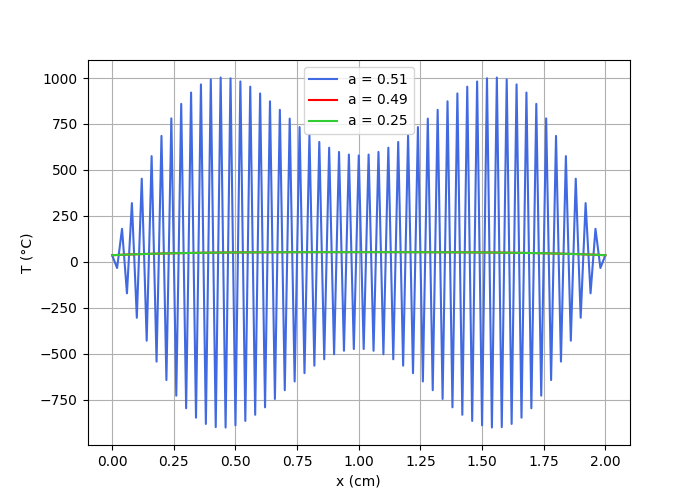
\includegraphics[width=\textwidth]{inestable.png}
    \end{minipage}
    \hfill
    \begin{minipage}{0.47\textwidth}
        \centering
        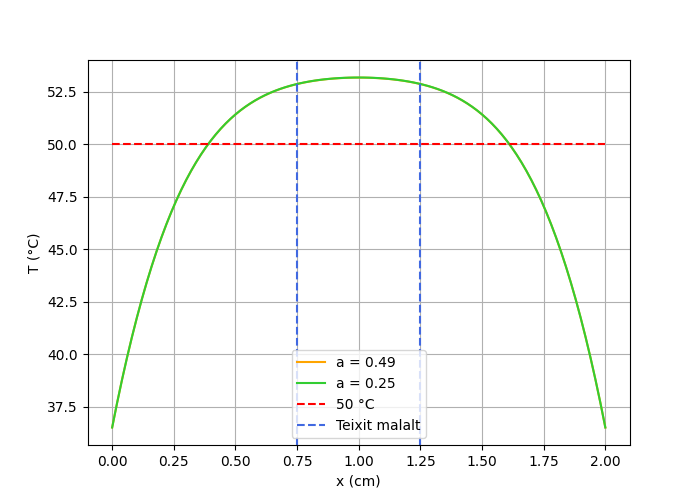
\includegraphics[width=\textwidth]{estable.png}
    \end{minipage}

    \caption{Representació gràfica de la temperatura en funció de l'espai. La figura de l'esquerra mostra els tres mallats 
    temporals mentre que la figura de la dreta suprimeix el mallat per a $a = 0.51$, per facilitar l'observació de la 
    representació dels altres dos mallats temporals.}
    \label{figura1}

\end{figure}


A la figura \ref{figura1} es pot observar que els resultats obtinguts amb els passos temporals 
$\Delta \widetilde{t} = 0.49(\Delta \widetilde{x})^2$ i $\Delta \widetilde{t} = 0.25(\Delta \widetilde{x})^2$ són tan 
propers entre si que presenten una superposició visual. En canvi, quan s'utilitza $\Delta \widetilde{t} = 0.51(\Delta \widetilde{x})^2$, la solució presenta un 
comportament oscil·latori, el que ens indica un comportament inestable i físicament incoherent, amb temperatures que fins i tot arriben a 
valors inferiors a $0\,\mathrm{K}$.

Aquesta diferència s'explica per l'estabilitat del mètode d'Euler explícit, que depèn del mallat emprat. En concret, 
pel nostre cas cal que el pas temporal compleixi la condició $\Delta \widetilde{t} \leq 0.5(\Delta \widetilde{x})^2$. 
Per tant, els dos primers mallats compleixen aquesta condició i proporcionen resultats estables, mentre que el tercer la supera 
i provoca la divergència de la solució numèrica.

\begin{figure}[h]
    \centering

    \begin{minipage}{0.47\textwidth}
        \centering
        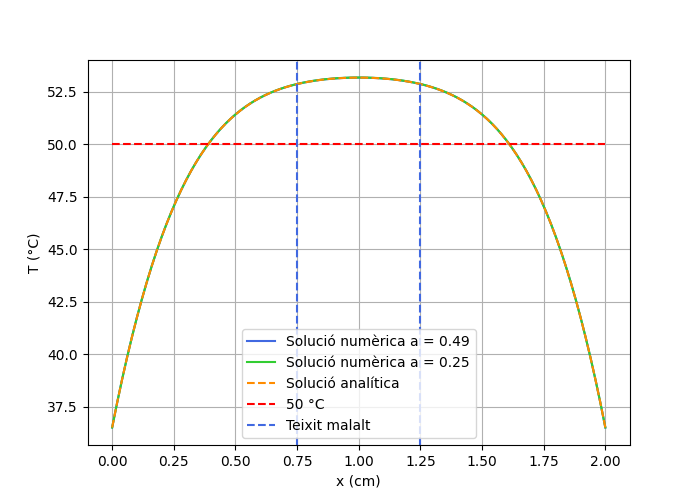
\includegraphics[width=\textwidth]{numerica_analitica.png}
    \end{minipage}
    \hfill
    \begin{minipage}{0.47\textwidth}
        \centering
        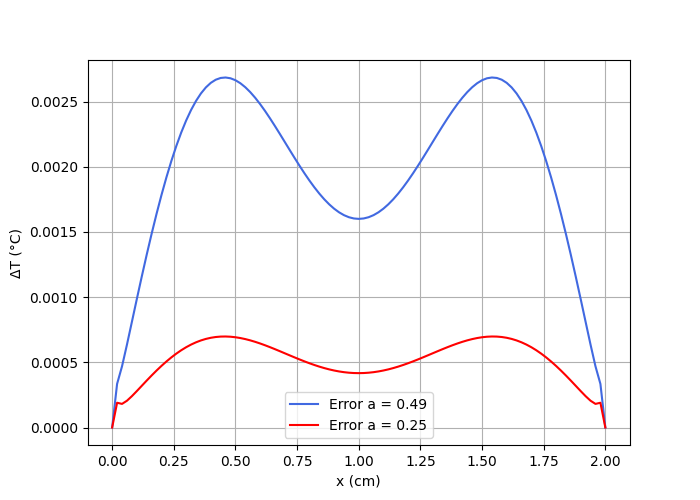
\includegraphics[width=\textwidth]{errores.png}
    \end{minipage}

    \caption{A la figura de la dreta podem apreciar la comparació entre la solució analítica i la solució numèrica pels mallats 
    temporals amb $a$ igual a 0.49 i 0.25. A la figura de la dreta podem veure els errors numèrics d'aquests dos mallats en comparar-los 
    amb la solució analítica.}
    \label{figura2}

\end{figure}

Ara, avaluem l'error. A  la figura \ref{figura2} podem apreciar que les solucions per 
$\Delta \widetilde{t} = 0.49(\Delta \widetilde{x})^2$ i $\Delta \widetilde{t} = 0.25(\Delta \widetilde{x})^2$ són molt properes entre si i properes amb la solució analítica, 
tal i com demostra l'ordre de magnitud de l'error. També podem observar que, tal com és d'esperar, quan disminuïm l'amplada del 
mallat i augmentem el nombre de punts, l'error disminueix. Donat que hem obtingut una diferència màxima de temperatura 
$\Delta T < 0.003$ respecte la solució analítica, i recordant que estem treballant amb temperatures al voltant dels 50 $^\circ$C 
considerem que es tracta d'un error acceptable i, així doncs, d'uns resultats numèrics força precisos.

En cas de no conèixer la solució analítica, podríem comprovar que el programa va bé modificant el mallat temporal. Si 
el programa funciona correctament hauria de convergir cap a una solució en disminuir l'amplada del mallat temporal i, en 
conseqüència, augmentant el nombre de punts. 


\subsection{Euler implícit}


\begin{figure}[h]
    \centering
    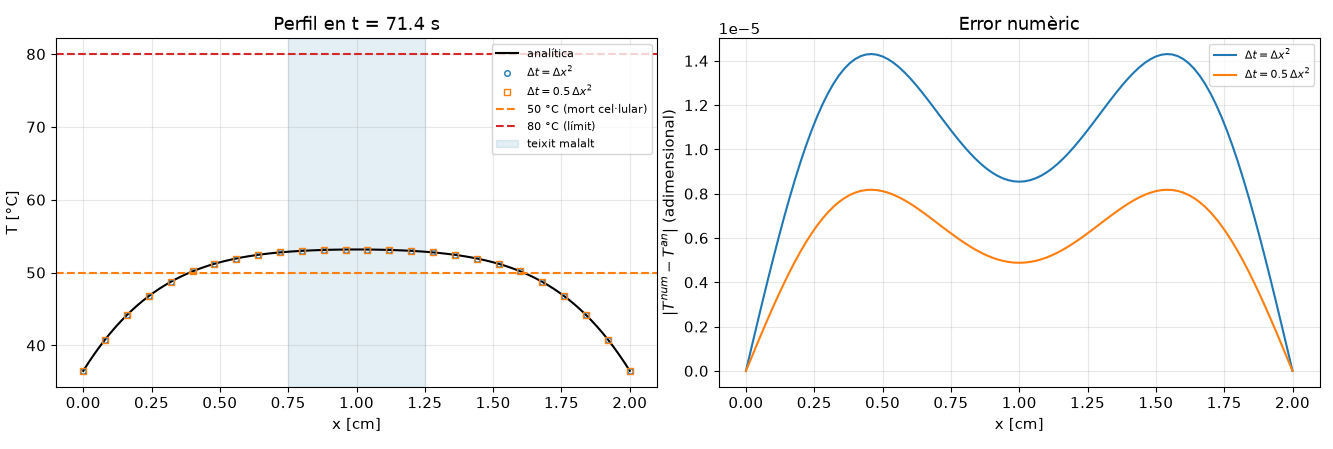
\includegraphics[width=0.97\textwidth]{euler_implicito.png}

    \caption{A la figura de l'esquerra es mostra el perfil de temperatura en funció de l'espai per a $t = 71.4\,\mathrm{s}$, 
    comparant la solució analítica amb la solució numèrica obtinguda amb el mètode d'Euler implícit per als mallats 
    temporals $\Delta \widetilde{t} = (\Delta \widetilde{x})^2$ i $\Delta \widetilde{t} = 0.5(\Delta \widetilde{x})^2$. A la figura 
    de la dreta es representa l'error numèric punt a punt d'aquests dos mallats respecte a la solució analítica.}
    \label{figura3}

\end{figure}

A la figura \ref{figura3} es pot observar que els resultats obtinguts amb el mètode d'Euler implícit pels dos mallats 
temporals coincideixen visualment amb la solució analítica. El perfil és simètric respecte al centre de la paret, on s'assoleix 
la temperatura màxima, que és d'aproximadament $53.17\,^\circ\mathrm{C}$. Aquest valor supera el llindar de mort cel·lular de 
$50\,^\circ\mathrm{C}$ però es manté clarament per sota del límit de $80\,^\circ\mathrm{C}$ a partir del qual es 
podria formar trombosi. A diferència del mètode explícit, aquí no apareix cap oscil·lació, ni tan sols amb 
$\Delta \widetilde{t} = (\Delta \widetilde{x})^2$, que supera el límit $\Delta \widetilde{t} \leq 0.5(\Delta \widetilde{x})^2$ 
d'estabilitat de l'Euler explícit. Això és coherent amb el fet que el mètode d'Euler implícit és incondicionalment estable, de manera 
que la tria del pas temporal només condiciona la precisió i no l'estabilitat de la solució.

Ara, avaluem l'error. Tal i com es veu a la figura \ref{figura3}, l'error és nul als extrems, on s'imposa la condició de contorn, 
i assoleix el màxim a prop de $x \approx 0.46\,\mathrm{cm}$ (i, per simetria, de $x \approx 1.54\,\mathrm{cm}$). Per a 
$\Delta \widetilde{t} = (\Delta \widetilde{x})^2$ l'error màxim és de $1.4 \cdot 10^{-5}$ en unitats adimensionals, mentre que 
per a $\Delta \widetilde{t} = 0.5(\Delta \widetilde{x})^2$ és de $8.2 \cdot 10^{-6}$. Així, tal i com és d'esperar, quan 
disminuïm el pas temporal l'error disminueix, tot i que el factor de reducció és d'aproximadament $1.75$ i no $2$, el que indica 
que a més de l'error de truncament temporal també hi ha una contribució de l'error de discretització espacial, que és el mateix 
en els dos casos. Si tornem a les unitats físiques, aquests errors corresponen a diferències de temperatura 
$\Delta T \approx 0.010\,\mathrm{K}$ i $\Delta T \approx 0.006\,\mathrm{K}$, respectivament, que són molt petites 
comparades amb una temperatura de l'ordre de $50\,^\circ\mathrm{C}$. Per tant, considerem que es tracta d'un error 
acceptable i que els resultats numèrics són força precisos.




\subsection{Crank-Nicolson}

A continuació, es comparen els resultats amb la solució analítica i s'analitza l'error comès.

\begin{figure}[h]
    \centering
    \begin{minipage}{0.45\textwidth}
        \centering
        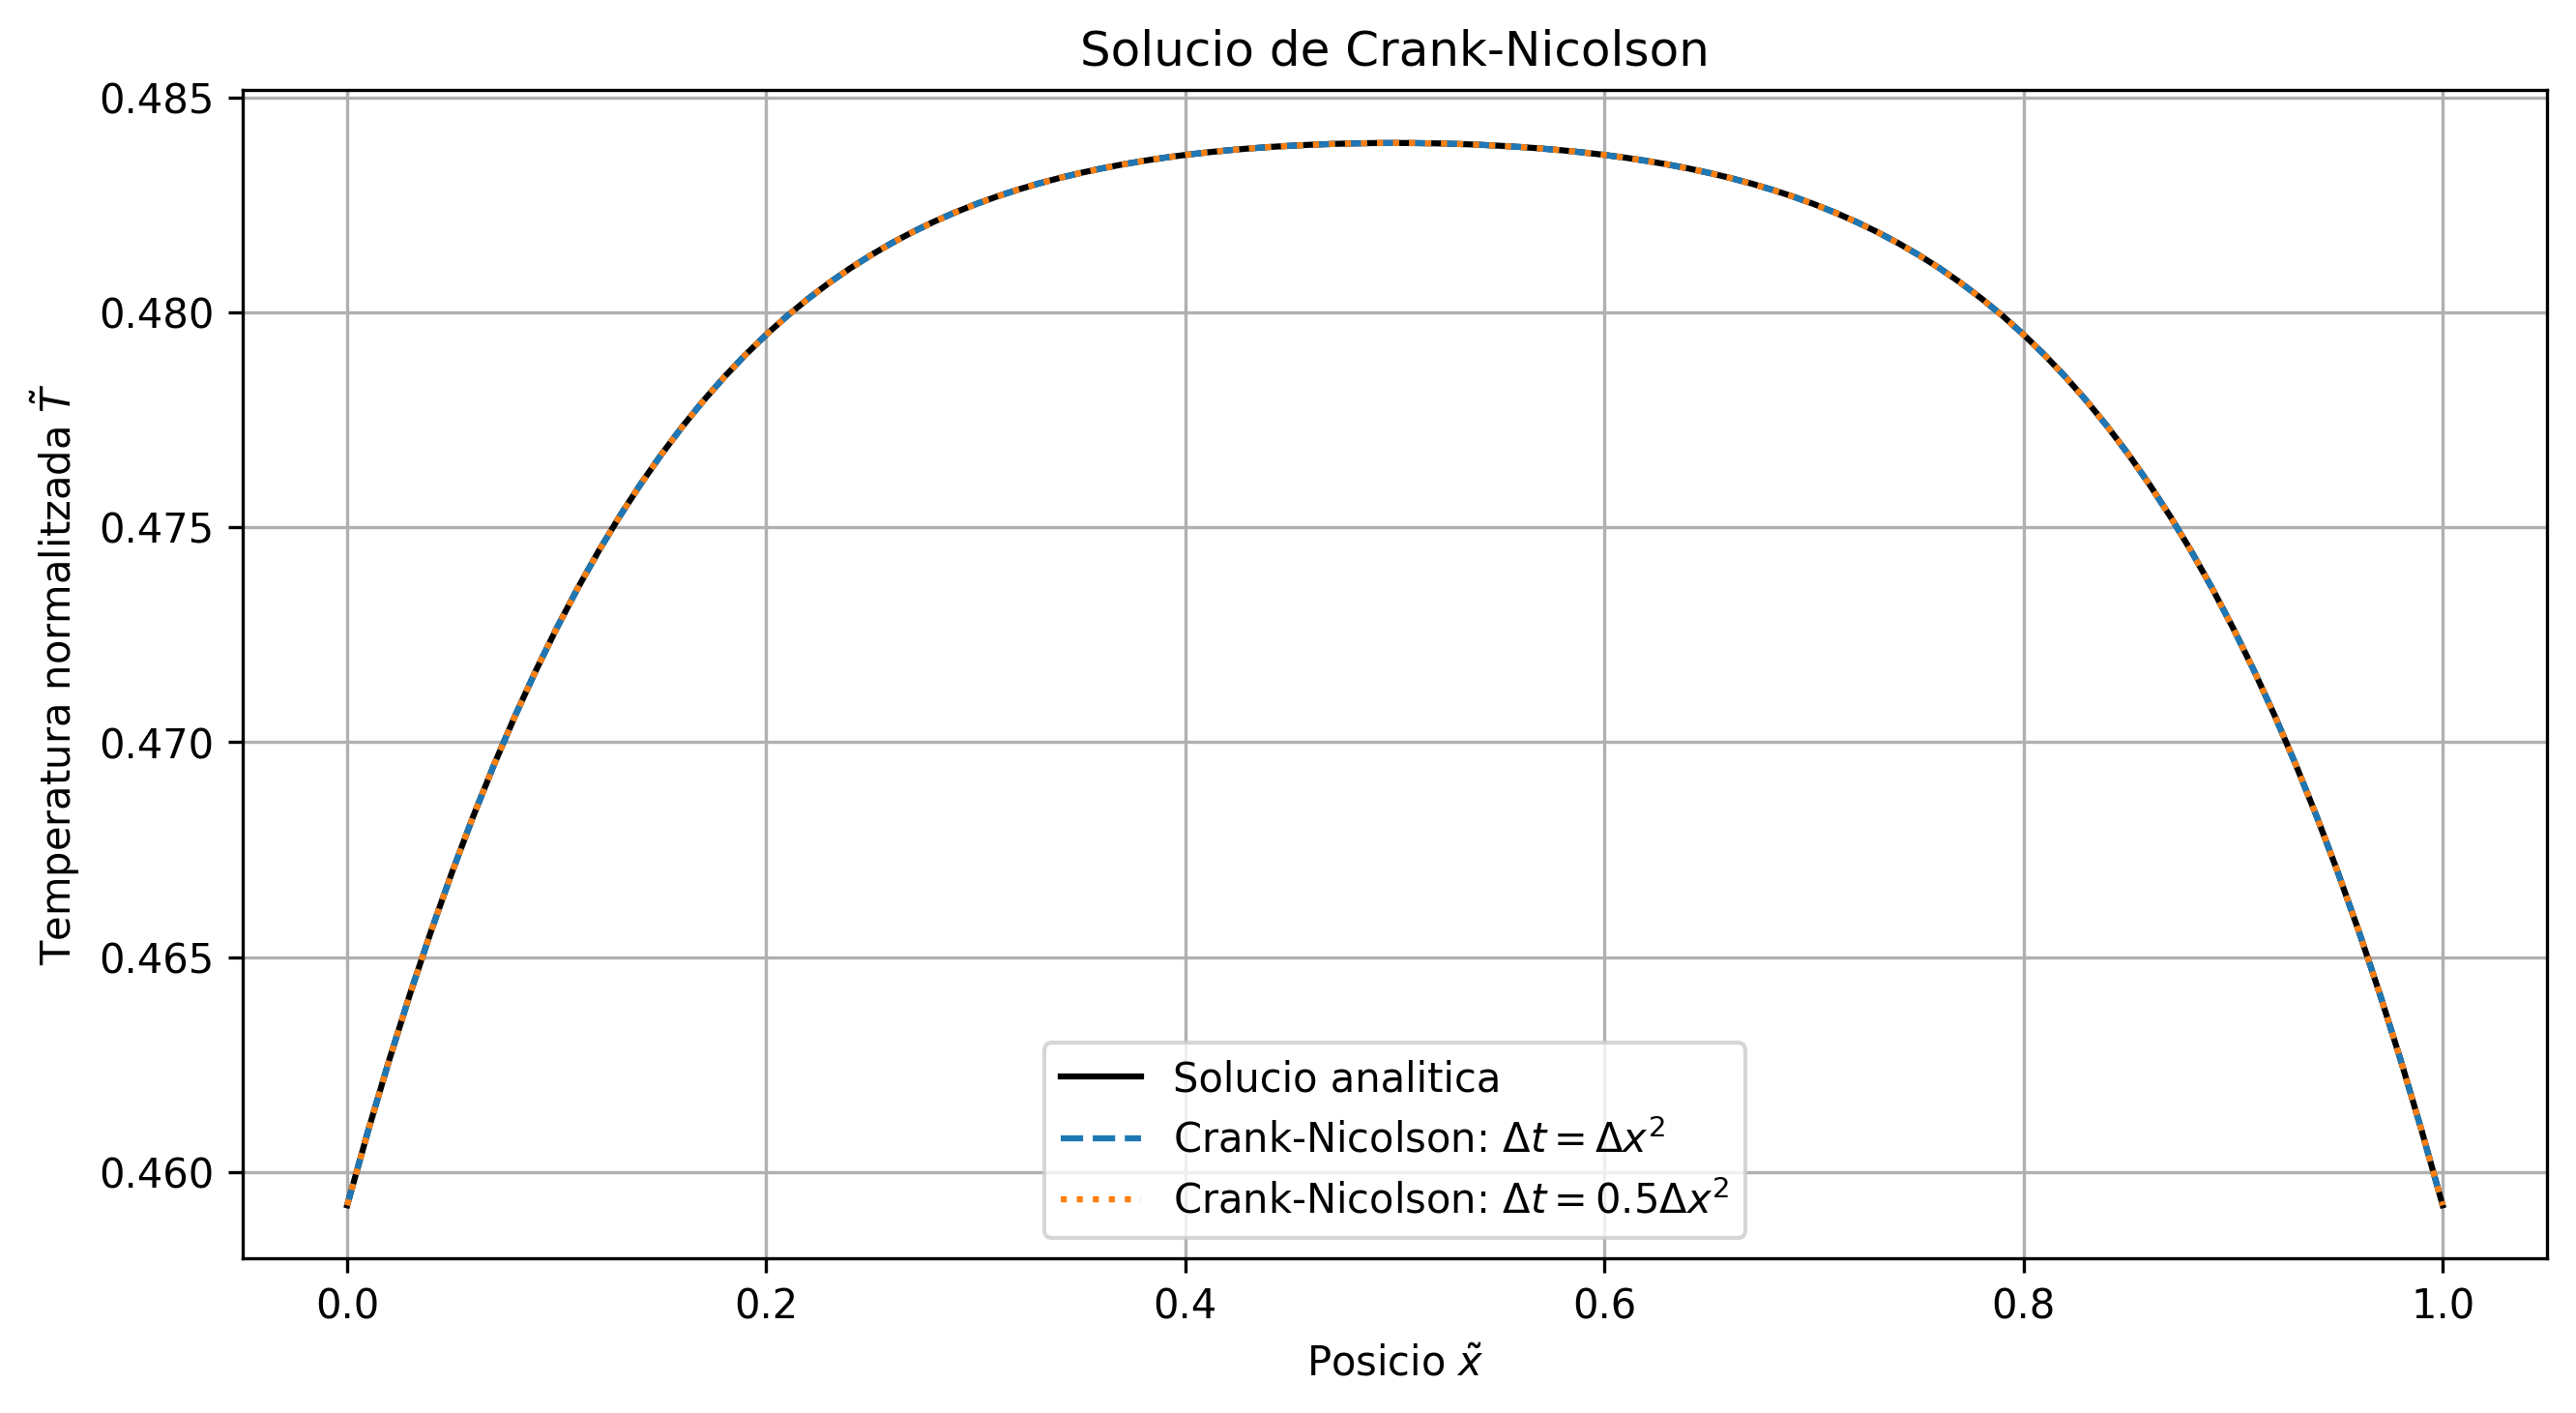
\includegraphics[width=\textwidth]{grafica_temperatures.png}
        \caption{Comparació entre la solució analítica i les dues solucions numèriques obtingudes amb el mètode de Crank-Nicolson.}
        \label{fig 1}
    \end{minipage}
    \hfill
    \begin{minipage}{0.45\textwidth}
        \centering
        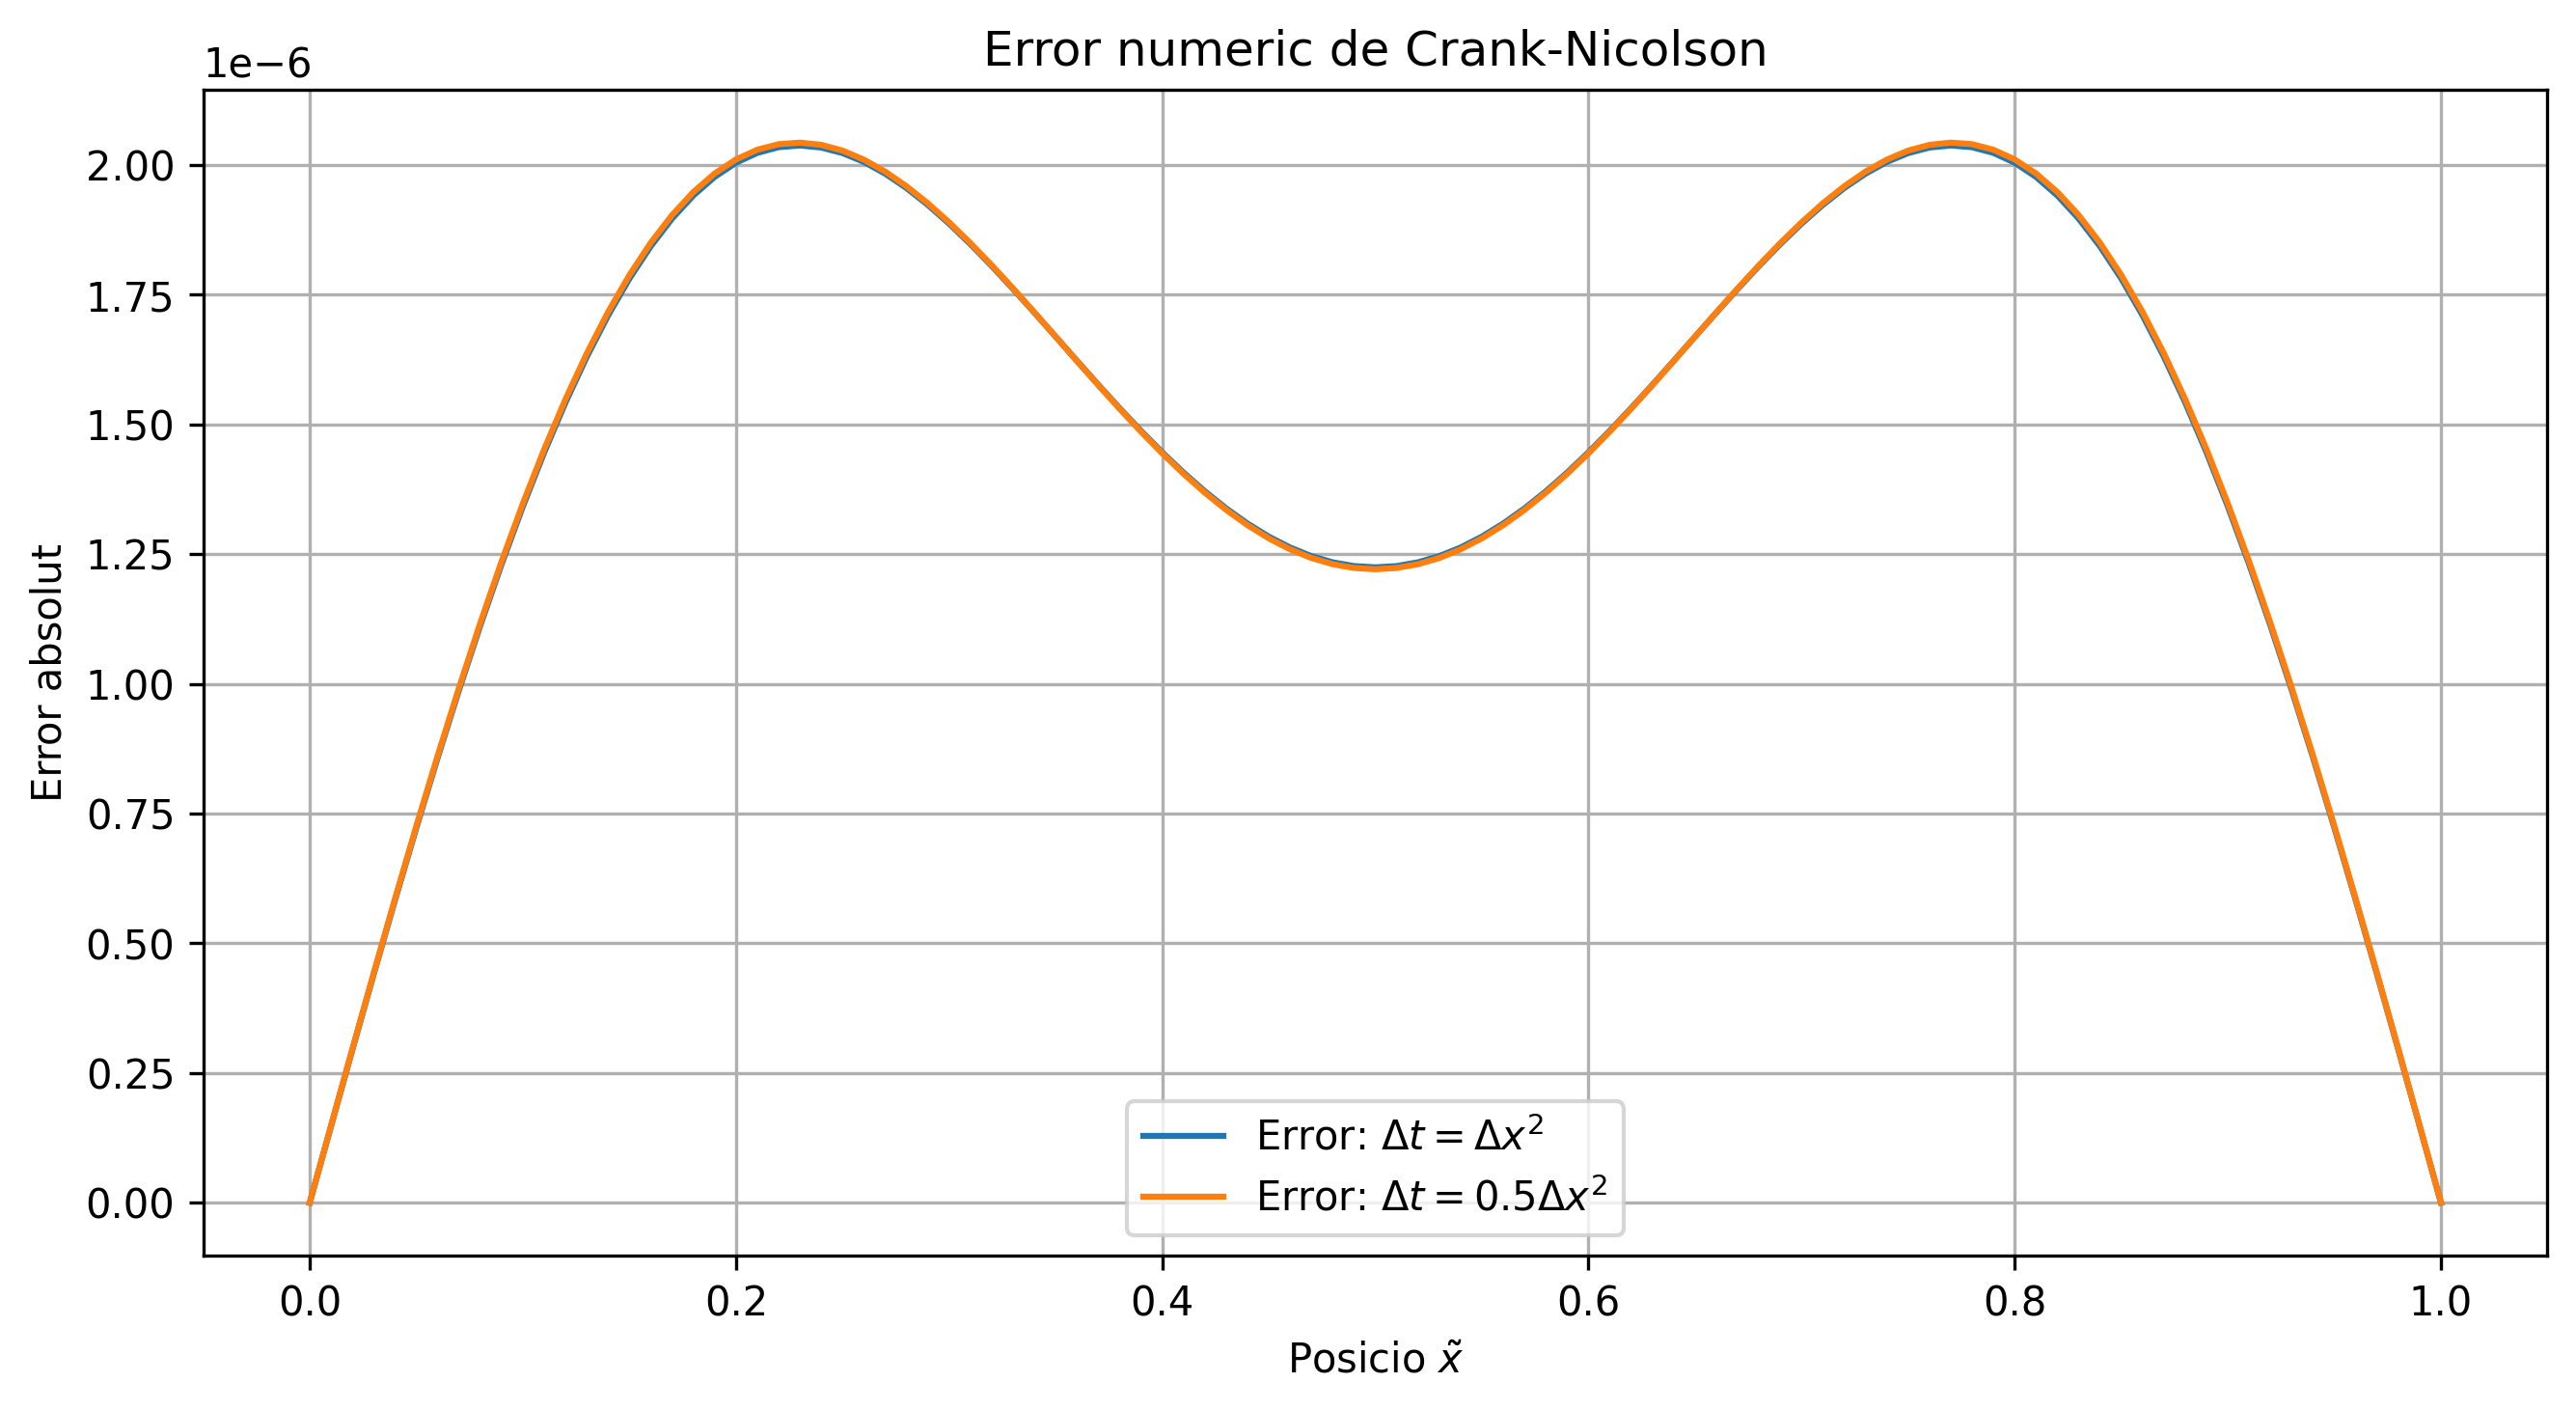
\includegraphics[width=\textwidth]{grafica_errors.png}
        \caption{Error absolut de les dues solucions numèriques respecte de la solució analítica.}
        \label{fig 2}
    \end{minipage}
\end{figure}

A la figura \ref{fig 1} es representen les tres solucions obtingudes. Com es pot observar, les dues aproximacions numèriques 
pràcticament coincideixen amb la solució analítica, fins al punt que les tres corbes se superposen gairebé completament.

Per comprovar amb més detall la precisió dels resultats, hem representat l'error absolut entre les solucions numèriques i 
l'analítica. A la figura \ref{fig 2} es pot observar que els errors són molt petits, ja que es mantenen al voltant de 
l'ordre de \(10^{-6}\). Com es pot veure, reduir el pas temporal a la meitat i duplicar el nombre de passos, passant de 250 a 500, no suposa una 
millora en la precisió. De fet, el segon cas presenta un error lleugerament més gran, tot i que la diferència entre tots dos 
és pràcticament negligible.

Per tant, en aquest cas, el primer pas temporal resulta més convenient, ja que permet obtenir una precisió molt similar amb 
la meitat de passos temporals i, per tant, amb un menor cost computacional.

\begin{figure}[h]
    \centering
    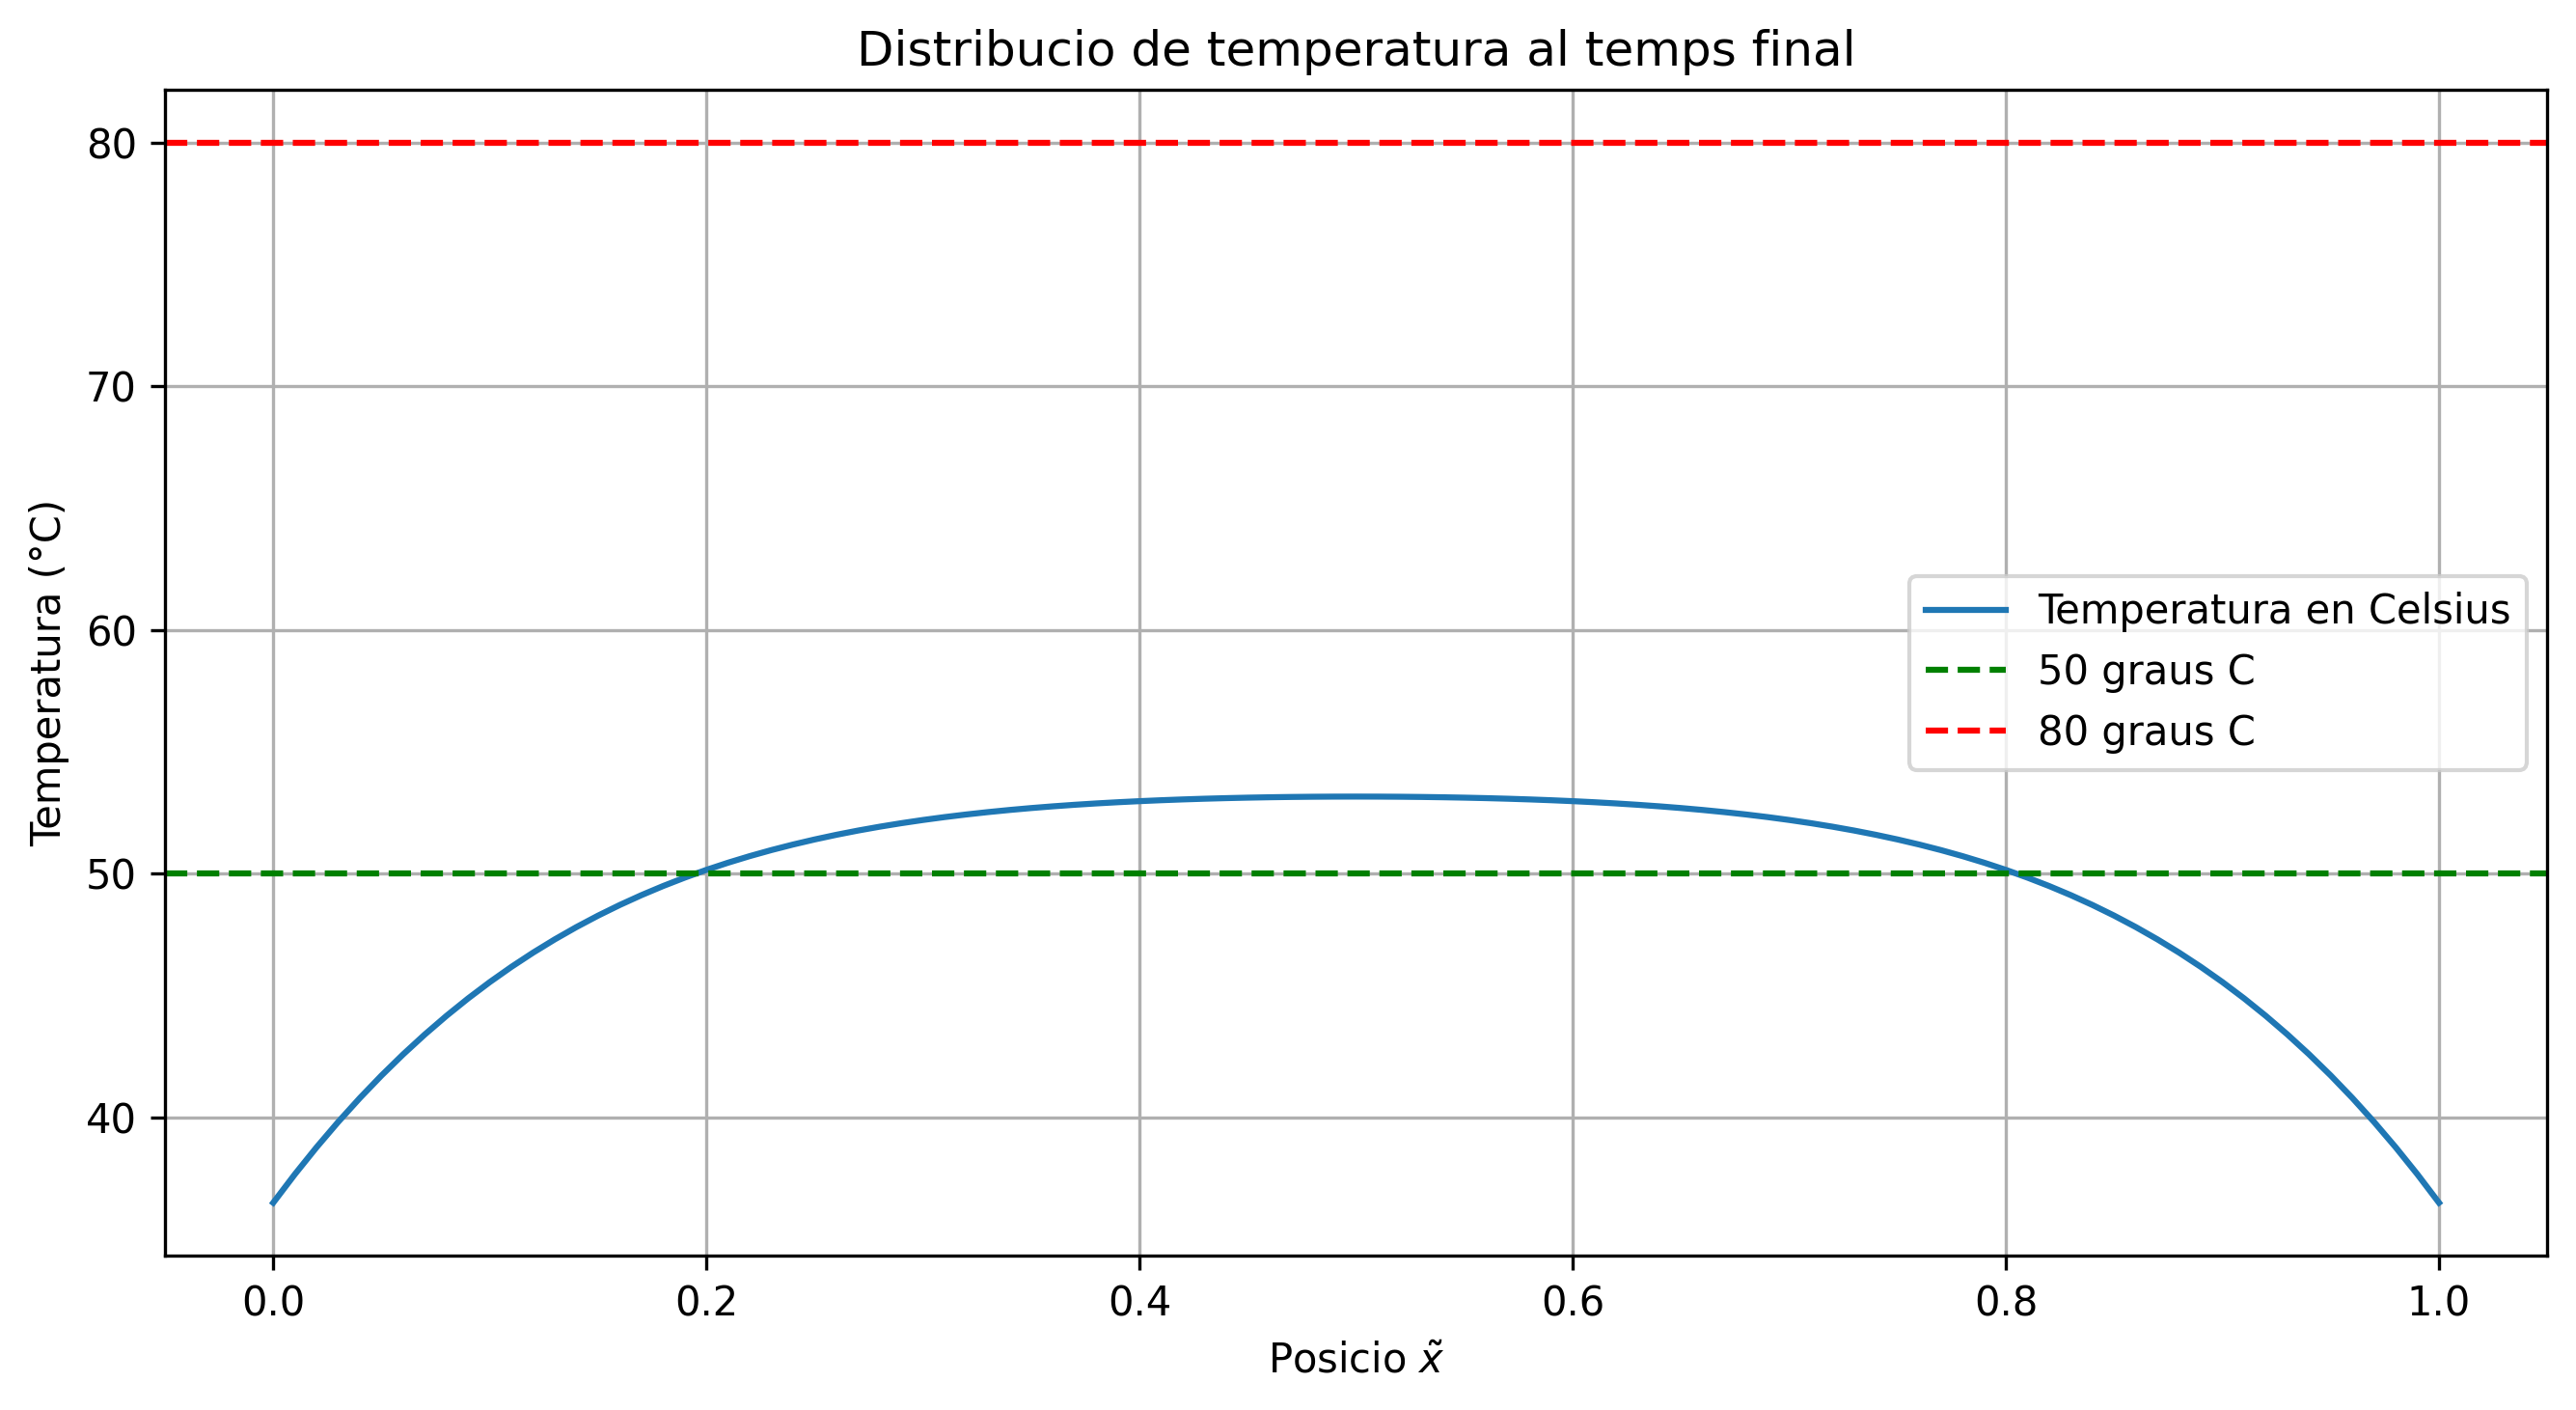
\includegraphics[width=0.5\linewidth]{grafica_celsius.png}
    \caption{Distribució de la temperatura en graus Celsius al temps final de la simulació. Les línies discontínues indiquen els límits de 50 °C i 80 °C.}
    \label{fig 3}
\end{figure}


La gràfica \ref{fig 3} mostra que la temperatura arriba a un màxim aproximat de $53\,^\circ\mathrm{C}$ al centre del domini. 
Tota la regió malalta ($0.375\leq\tilde{x}\leq0.625$) supera els $50\,^\circ\mathrm{C}$ sense arribar als $80\,^\circ\mathrm{C}$, 
de manera que es compleixen els dos primers objectius del tractament. Llavors, podem afirmar que el mètode de 
Crank-Nicolson proporciona resultats prou precisos per als dos passos temporals estudiats.


\subsection{Comparació dels mètodes d'Euler explícit, Euler implícit i Crank-Nicolson}
 

\begin{figure}[h]
    \centering
    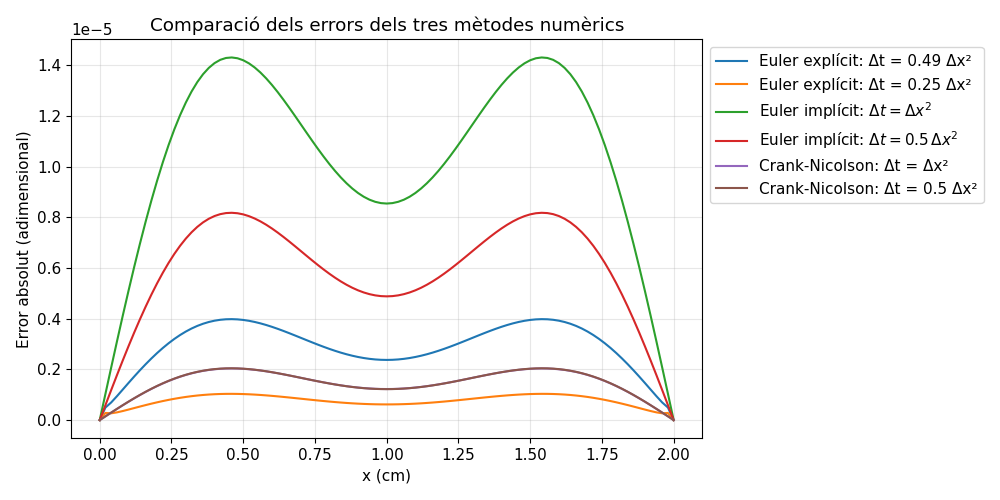
\includegraphics[width=0.7\linewidth]{comparacio_error.png}
    \caption{Comparació dels errors dels mètodes d'Euler explícit, implícit i Crank-Nicolson}
    \label{comparacio}
\end{figure}

Segons la gràfica de la figura \ref{comparacio}, observem que el mètode d'Euler explícit amb $a=0.25$ és el que ofereix un menor 
error numèric. Això es deu al fet que utilitza un pas temporal més petit que els altres mètodes i, per tant, redueix l'error de 
discretització temporal i permet obtenir una aproximació més precisa de la solució analítica. Per tant, tot i que els mètodes 
implícits són estables, en aquest cas l'Euler explícit amb $a=0.25$ proporciona els resultats més precisos.

\section{Resolució del problema}

Utilitzant el mètode d'Euler explícit, hem pogut determinar que el temps que cal aplicar el senyal de 40 V per tal que la regió 
malalta assoleixi una temperatura entre 50 $^\circ$C i 80 $^\circ$C sense que el teixit sa arribi als 50 $^\circ$C i sense que 
cap regió sobrepassi els 80 $^\circ$C és de: $t = 58.34406711000042$ s. 

\section{Propostes per millorar el model}

Es podria millorar el model de la potència externa $P_{\mathrm{ext}}$ considerant els efectes de vorada dels elèctrodes, 
ja que en el model actual es considera una distribució idealitzada i uniforme de la potència. En realitat, la potència dissipada 
per efecte Joule pot variar espacialment a causa de la geometria finita dels elèctrodes.

Per tenir en compte aquest efecte, es podria ampliar el model a dues dimensions i considerar una diferència de potencial 
efectiva dependent de la posició, $\Delta V(x,y)$. Això permetria definir una potència externa variable espacialment, 
$P_{\mathrm{ext}}(x,y)$, i incorporar-la a l'equació de la calor:

\[
c_v\rho\frac{\partial T}{\partial t}
= \kappa\left(\frac{\partial^2 T}{\partial x^2} + \frac{\partial^2 T}{\partial y^2}\right) + P_{\mathrm{ext}}(x,y)
\]

Així, es podria representar de manera més realista la distribució de calor dins del teixit, incloent-hi les variacions de 
potència causades pels efectes de vora.

Altres propostes més complexes podrien ser considerar la pèrdua de calor produïda per la circulació de sang i pel contacte amb 
altres teixits i òrgans, o que la calor produïda per efecte Joule pugui variar amb el temps depenent de les propietats elèctriques 
dels teixits.

\section{Conclusions}

En aquesta pràctica hem modelitzat la transferència de calor durant una ablació cardíaca mitjançant l'equació de Fourier i 
hem simplificat l'estudi amb una normalització. Hem implementat tres mètodes numèrics: Euler explícit, Euler implícit i 
Crank-Nicolson; i hem comparat l'estabilitat i la precisió amb la solució analítica.

Els resultats mostren que l'Euler explícit només és estable per determinats mallats temporals (el criteri d'estabilitat és $\Delta \widetilde{t} = 0.51(\Delta \widetilde{x})^2$), 
mentre que els mètodes implícits no presenten aquesta restricció. En general, els tres mètodes ofereixen resultats precisos, amb 
errors numèrics petits, tot i que cal destacar que el mètode d'Euler explícit ha sigut el que ha proporcionat un error menor. 
Per aquest motiu, hem estimat amb aquest mètode un temps de tractament d'aproximadament \(58.34\,\mathrm{s}\) per assolir les 
temperatures desitjades a la zona malalta, sense superar els \(80\,^\circ\mathrm{C}\). També hem identificat limitacions del 
model, com la distribució uniforme de la potència i l'absència de pèrdues de calor, que es podrien millorar incorporant els 
efectes dels elèctrodes i la circulació sanguínia.



\newpage

\section{Contribucions i ús d'IA}

\subsection{Contribucions}

Per l'elaboració de la pràctica ens hem dividit la feina de tal forma que cada membre del grup s'encarrega d'un mètode numèric 
diferent. Cada membre del grup ha trobat l'algorisme del seu mètode, l'ha implementat en Python i ha redactat la part teòrica 
del mètode i els resultats obtinguts. El Víctor s'ha encarregat del mètode d'Euler explícit i la comparació dels errors, 
el Gabriel de l'implícit i l'Aleix del Crank-Nicolson. El Gabriel ha calculat la solució analítica de l'equació diferencial. 
A la redacció de l'informe, el Víctor ha redactat la introducció teòrica de la pràctica (excepte els subapartats dels mètodes 
implícits), les parts corresponents a l'Euler explícit i la comparació d'errors, el Gabriel ha escrit les parts corresponents a 
l'Euler implícit i l'Aleix s'ha encarregat de les parts corresponents al Crank-Nicolson i ha fet les conclusions.



\subsection{Ús d'IA}

Hem utilitzat ChatGPT com a eina de suport durant el desenvolupament de la pràctica, principalment per 
recerca bibliogràfica per resoldre dubtes sobre els mètodes numèrics, revisió ortogràfica i per assistir en la detecció d'errors 
de compilació en els codis, principalment el LaTex. També per consultar ràpidament com representar algun símbol a LaTex quan no 
recordàvem o no sabíem quina era la seva comanda.

Els codis, els resultats obtinguts i la seva interpretació han estat elaborats íntegrament pels membres del grup, que són responsables del 
contingut final del treball. 

Considerem que la IA ha sigut una eina de suport que ha servit per agilitzar el desenvolupament de la pràctica, donat que en 
alguns casos no érem capaços d'identificar quin era el motiu pel qual el document de l'informe no compilava o per trobar símbols. 
Tot i això, considerem que sense cap eina d'IA seríem capaços de realitzar d'igual forma aquesta pràctica, malgrat que seria un 
procés més lent.





\newpage

\section{Referències}
\textsc{escartín, j. m., \& navau, c.} (2026),
\textit{Mètodes numèrics II: Apunts de l'assignatura. Teoria} (versió 2.1.0). Universitat Autònoma de Barcelona
\\
\\
\textit{Enunciat pràctica 1: Modelització del tractament d'ablació cardíaca IVS} (2026). Universitat Autònoma de Barcelona

\section{Annex}
Els codis que hem fet servir per elaborar aquesta pràctica es troben en un repositori públic de GitHub. Aquí hi ha un enllaç 
al repositori: \color{blue} \href{https://github.com/Victor-sli/Codis-practica1-Grup-G111}{Codis Grup G111}. \color{black}



\end{document}
